\cleardoublepage
\chapter{Koopmans functionals for periodic systems\label{ch:koopmans-periodic}}
In the previous chapter we described the general framework of Koopmans functionals, without focusing on the specific issues that arise when passing from finite to extended systems. Here, we address the issues that are particularly relevant when dealing with infinitely periodic systems, where the need for a localized set of orbitals brings about the apparent breaking of the translation symmetries of the system. The chapter is organized as follows: in Sec.~\ref{sec:localization}, we bring up the importance of having localized sets of variational orbitals in Koopmans functionals and Wannier functions are introduced; in Sec.~\ref{sec:bloch-theorem}, we discuss the validity of Bloch's theorem in the framework of ODD functionals, which represents one of the main results of this thesis; finally, Sec.~\ref{sec:koopmans-pbc} is devoted to the formulation of Koopmans functionals in periodic boundary conditions. As usual, we close with a small section that summarizes the content of the chapter.

Part of the content of this chapter has been published in Refs.~\cite{de_gennaro_blochs_2022} and \cite{colonna_koopmans_2022}.

\clearpage
\section{The importance of localization\label{sec:localization}}
Two important aspects underlie the forthcoming discussion about the localization in Koopmans functionals: (i) the discussion at the end of Sec.~\ref{sec:deriv-dis}, and (ii) the nature of the KI correction [see Eq.~\eqref{eq:ki-correction}]. The effects of the orbitals localization on the derivative discontinuity and on the PWL were already touched upon, whereas the impact that such effects can have in infinitely periodic systems, and how they affect Koopmans corrections is the topic of this section.

As usual, we start from standard DFT. It is known that local and semi-local DFAs tend to spread the orbitals as much as possible over the whole system's extension. This is a consequence of the self-interaction error or, equivalently, the deviation from the PWL that affects such approximations, to the point that it was suggested by Mori-S\'{a}nchez \emph{et al.} to interpret the failures of local functionals in terms of a \emph{delocalization error} \cite{mori-sanchez_localization_2008}. The orbitals delocalization modifies the way the energy deviates from the exact PWL behavior\footnote{Once more, we remark that a correct PWL consists of two equally important features: (i) the linear trend at fractional occupations, and (ii) the correct estimation of the energies on either side of each linear segment, namely the energies at integer numbers of electrons. The fulfillment of the first requirement only, brings to a curve which is, indeed, piecewise-linear, but without the correct slope of the linear segments; in this sense, we consider such a curve to be deviating from the (exact) PWL behavior.}: for finite systems -- the limited extension of the system does not let the orbitals to delocalize too much -- the energy profile is the one showed in the red curve of Fig.~\ref{fig:deviation-pwl}, where the energies at integer points are quite correct, while at fractional occupation we observe a mistaken non-linear convex trend; by increasing the size of the system, the orbitals delocalization increases and the non-linear trend progressively turns into a linear one, while the relative position of the energies at integer numbers of electrons decreases (as shown in Fig.~\ref{fig:pwl-solids}). Such behavior is a natural consequence of the convexity of approximated energy functionals: if we consider a periodic system made of $M$ repetitions of the unit cell, each of which contains $N$ electrons, and we imagine to add a fraction of an electron $\delta$, Eq.~\eqref{eq:convexity} shows that local functionals will split the electron -- equally, in order to preserve the translation symmetry of the system -- among the different unit cells. The total ground-state energy of the system then reads as \cite{mori-sanchez_localization_2008}
%
\begin{equation}
    \begin{split}
    E^{\rm DFA}(NM + \delta) &= M E^{\rm DFA}\left( N + \frac{\delta}{M} \right) \\
    &= ME(N) + \delta \left. \frac{dE^{\rm DFA}}{dN} \right|_{N+\delta} + \mathcal{O} \left( \frac{\delta^2}{M} \right) .
    \end{split}
    \label{eq:pwl-convex-to-linear}
\end{equation}
%
When approaching the thermodynamic limit ($M\longrightarrow \infty$), the dependence of the energy on $\delta$ becomes more and more linear, reflecting the trend showed in Fig.~\ref{fig:pwl-solids}. Moreover, thanks to Janak's theorem
\footnote{The \emph{aufbau} principle tells us that the change in the ground-state energy due to a variation in the number of particles, is equivalent to the one coming from a variation in the occupation of the HO orbital; the Janak's theorem for the HO orbital can then be rewritten as a derivative with respect to the total number of particles:
\begin{equation*}
    \frac{dE}{dN} = \frac{dE}{df_{\rm HO}} = \varepsilon_{\rm HO} .
\end{equation*}
},
Eq.~\eqref{eq:pwl-convex-to-linear} shows that the derivative of the energy equals the KS highest-occupied eigenvalue, which strongly underestimates the IP of the system. To summarize, when dealing with infinitely extended systems, the energy of local and semi-local density-functionals shows a linear trend that, at a first sight, might resemble the exact PWL behavior; however, it turns out that, differently from small finite systems where the orbitals remain localized and $\Delta$SCF-like calculations provide an accurate prediction of ionization energies, here the separation between energies at integer points is strongly underestimated, meaning that not only energy derivatives, but also total energy differences (where an electron was removed from, or added to, a delocalized KS orbital), miss completely the ionization energies of the system.

\begin{figure}
    \centering
    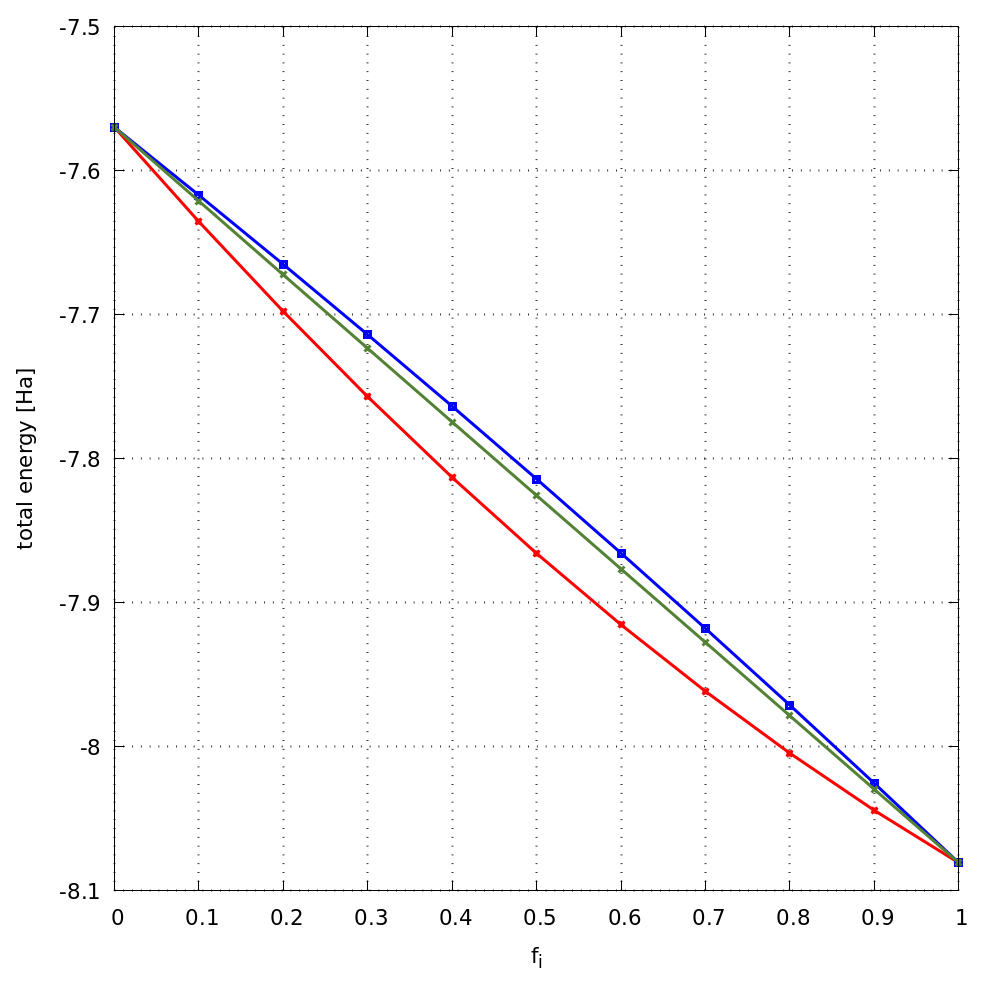
\includegraphics[width=0.5\linewidth]{ene-vs-occ-homo.png}
    \caption[]{}
    \label{fig:pwl-solids}
\end{figure}

The failure of local and semi-local DFAs to describe delocalized states becomes crucial when Koopmans corrections are introduced. As mentioned repeatedly, the KI correction linearizes the energy of the base functional at fractional occupations, and it retains it at integer points. Therefore, for a functional that is already linear, the $\Pi_i^{\rm KI}$ terms of Eq.~\eqref{eq:pi-term-general}, or Eq.~\eqref{eq:ki-correction}, are all identically zero. In order to have effective Koopmans corrections in extended systems, it is necessary to switch to a localized representation of the electronic states, where the energy does not vary linearly with respect to a change in the orbital occupations. Rather than considering the Bloch-like KS states, Koopmans functionals resort to sets of localized orbitals -- e.g., Wannier functions -- where the constrained energy differences due to a variation in the filling of such orbitals yields, presumably, good results.


\begin{figure}
    \centering
    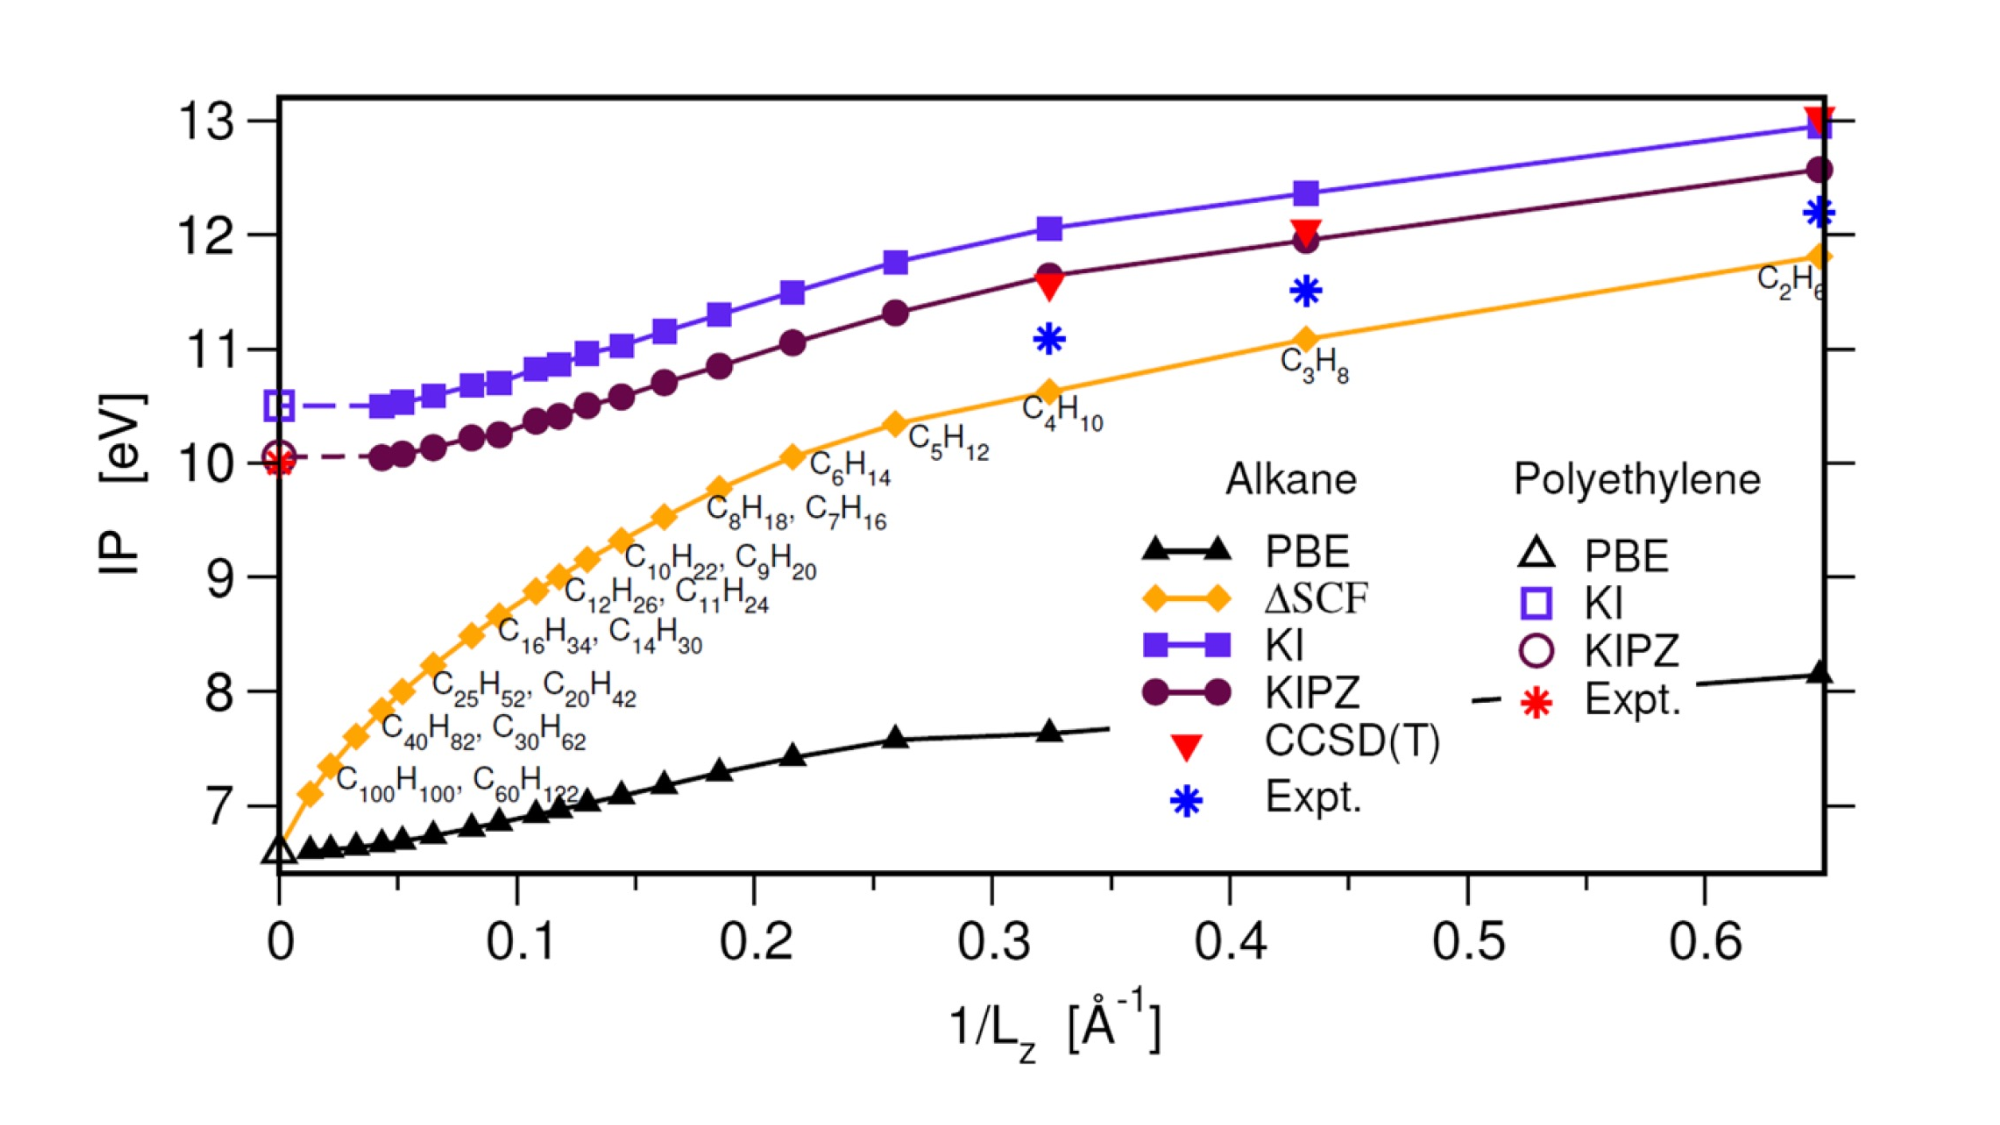
\includegraphics[width=0.8\linewidth]{IP-alkane-chain.pdf}
    \caption[]{Taken from Ref.~\cite{nguyen_koopmans-compliant_2018}.}
    \label{fig:ip-alkane-chain}
\end{figure}


\subsection{Wannier functions\label{sec:wannier-functions}}

\section{Bloch's theorem in ODD functionals\label{sec:bloch-theorem}}

\subsection{Bloch's theorem\label{sec:bloch-theorem-sub}}

\subsection{Validity in standard DFT\label{bloch-th-dft}}

\subsection{Validity in ODD functionals\label{sec:bloch-th-odd}}

\section{Koopmans functionals in periodic boundary conditions\label{sec:koopmans-pbc}}

\section{Summary\label{sec:ch4-summary}}

